\documentclass[11pt, oneside]{article} 	% use "amsart" instead of "article" for AMSLaTeX format
\usepackage{geometry} 		% See geometry.pdf to learn the layout options. There are lots.
\geometry{letterpaper} 		% ... or a4paper or a5paper or ... 
\usepackage[parfill]{parskip} 		% Activate to begin paragraphs with an empty line rather than an indent
\usepackage{graphicx}				% Use pdf, png, jpg, or eps§ with pdflatex; use eps in DVI mode
								% TeX will automatically convert eps --> pdf in pdflatex		
\usepackage{amssymb}
\usepackage{amsmath}
\usepackage{authblk}
\usepackage{framed}
\usepackage[
backend=biber,
style=alphabetic,
]{biblatex}
\usepackage{graphicx}
\graphicspath{ {./images/} }
\usepackage{verbatim}
\usepackage{tikz} 
\usepackage{subcaption}
\captionsetup{compatibility=false}



\usepackage{syntonly}

% \syntaxonly \langle -- use this for checking syntax only
% \mbox {text} - keep together	
% \fbox {text} - keep together and draw around

%\pagestyle{plain|headings|empty} % header and footer p.27
%SetFonts
%\include{filename}, \includeonly{filename1, filename2} , \input[fiename}

%SetFonts% 


\title{The Flags Problem}
\author{Dave Fetterman}
\affil{Obviously Unemployed}
\date{5/29/24}
\begin{document}
\maketitle

\begin{abstract}

This is a problem I thought about while driving around my town, yelling at pedestrians. Turning them into an abstraction proves useful here but it may not hold up in traffic court.


\end{abstract}

\section{The Problem}

Pedestrians are crossing a city street, either going left or right.
Orange handheld flags sit in racks on either side of the street to them to provide visibility to cars (Fig.~\ref{fig:flags0}).
If there is a flag in their side's rack, a pedestrian will take it across the street with them (Fig.~\ref{fig:flags1}) and place it in the opposite rack (Fig.~\ref{fig:flags2}).
If their side's rack is empty, they cross the street anyway and don't touch the flags (Fig.~\ref{fig:flags3}).


\begin{figure}[!htb]
\centering
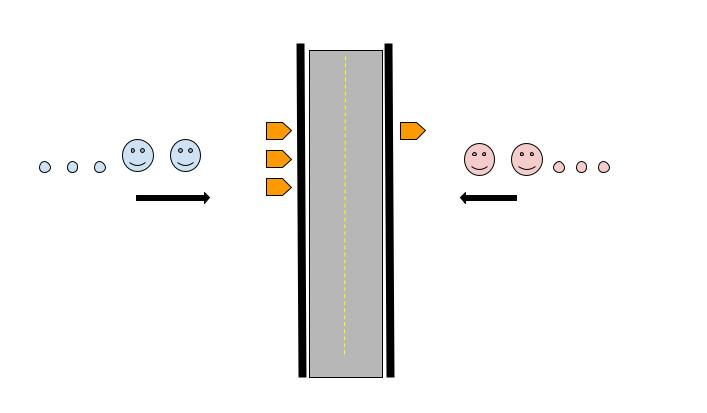
\includegraphics[scale=.3]{flags0}
\caption{Before Crossing}
\label{fig:flags0}
\end{figure}

\begin{figure}[!htb]
\centering
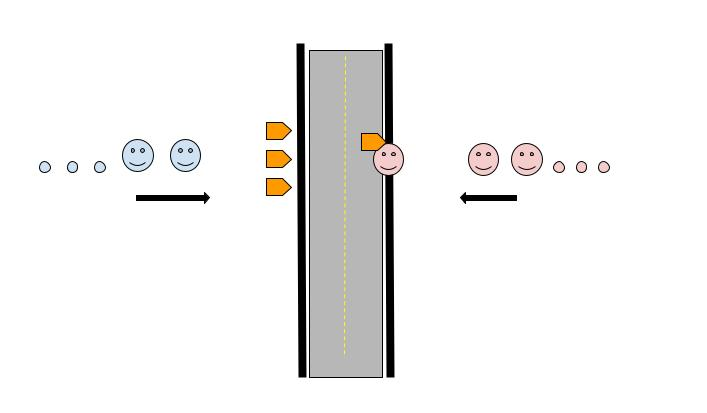
\includegraphics[scale=.3]{flags1}
\caption{Carry the flag}
\label{fig:flags1}
\end{figure}

\begin{figure}[!htb]
\centering
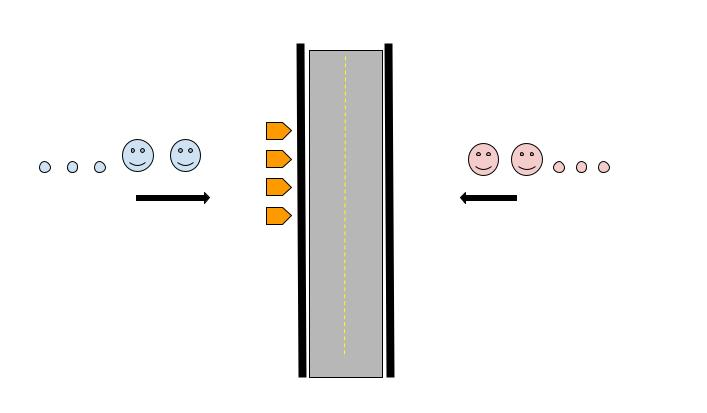
\includegraphics[scale=.3]{flags2}
\caption{After Crossing}
\label{fig:flags2}
\end{figure}

\begin{figure}[!htb]
\centering
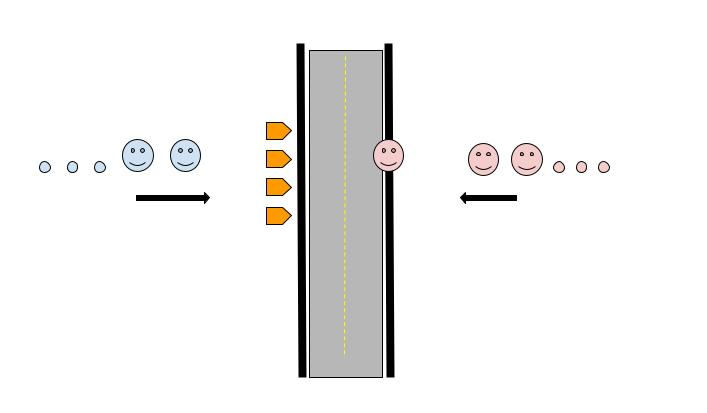
\includegraphics[scale=.3]{flags3}
\caption{Flagless Crossing}
\label{fig:flags3}
\end{figure}

We can assume:
\begin{itemize}
\item A very large number of pedestrians cross over the course of the day.
\item Pedestrians arrive and cross immediately, one at a time.
\item Pedestrians cross once, either right to left or left to right, and vanish for the rest of the day.
\item Each crossing is an independent event. The probability that the next pedestrian crosses left to right is some $p$, which doesn't change over the day.  Right-to-left is then $1-p$. 
\end{itemize}


\textbf{Questions}:
\begin{enumerate}
\item At the end of the day, suppose we see three flags on the left and one on the right.  What's the most likely value of $p$?\footnote{Given that we have no priors, we could call this the \emph{maximum likelihood estimate}. Or, the value of $p$ that makes this most probable.}
\item Suppose we see $k$ flags on the left and $n-k$ flags on the right.  What's the most likely value of $p$?
\end{enumerate}

\section{Solution}

\subsection{Markov Chain Model}

Rather than think of a line of pedestrians waiting to cross from either side, we should instead model this as a series of crossings from the left and right, with probabilities $p$ and $1-p$, respectively.  For example, the sequence $LRLLR$ would have probability $p(1-p)p^2(1-p)$.

To describe the flags, we also have states $A_0 ... A_n$, corresponding to 0 flags on the right side of the street, 1 flag on the right, up to $n$ flags on the right.  We denote the probability of being in state $A_k$ as $a_k$.  

\begin{figure}[!htb]
\centering
\begin{subfigure}{.5\textwidth}
 \centering
$ \left[\begin{array}{ccccc}
           1-p &1-p & 0 & 0 & 0 \\ 
           p & 0 & 1-p & 0 & 0 \\ 
           0 & p & 0 & 1-p & 0 \\ 
	  0 & 0 & p & 0 & 1-p \\ 
	  0 & 0 & 0 & p & p \\ 
           \end{array}\right] 
           \cdot
           \begin{bmatrix} a_0 \\ a_1 \\ a_2 \\ a_3 \\ a_4 \\
           \end{bmatrix}
           $
 \caption{Transition matrix from state $\vec{a}$}
\label{fig:markov}
\end{subfigure}
\end{figure}

Then, starting at time $t=0$ from state distribution vector $\vec{a}$, we can use a Markov model approach to describe the probability of being in each state at time $t=1$.  The matrix $M$ in Fig.~\ref{fig:markov}, when left-multiplied with state vector $\vec{a}$ at $t=0$, produces $\vec{a}$ at $t=1$.  $M_{ij}$, meaning the element in row $i$ and column $j$, gives the probability of transitioning from state $A_j$ to $A_i$.\footnote{Note that I zero-index matrices, a CS-based habit I've not been able to break} The first column, then, says that we have a $1-p$ probability of transitioning from state $A_0$ to $A_0$ (a flagless left crossing) and a $p$ probability of transitioning from state $A_0$ to $A_1$ (a crossing taking one of the $n-0 =  n$ flags on the left with us).

\subsection{Finding Equilibrium}

\begin{comment}
A Markov matrix will always have a largest eigenvalue of $\lambda  = 1$.  Though there are other proofs of this, since repeated application of the Markov chain will neither grow nor shrink a probability vector without bound, this must be so.  

With an eigenvalue $\lambda = 1$, this means we must have an eigenvector $\vec{a_\lambda}$ such that $M \cdot \vec{a_\lambda} = \lambda \cdot \vec{a_\lambda}$, or $M \cdot \vec{a_\lambda}  = \vec{a_\lambda}$.
\end{comment}

We assert without proof that $M$ is aperiodic (we're not going to get into a multi-step cycle, which seems clear), so by Markov chain theory, repeated application of $M$ will yield an equilibrium behavior no matter the initial state distribution $\vec{a}$. Therefore, we need to find an equilibrium solution as shown in Fig.~\ref{fig:equilibrium}.

\begin{figure}[!htb]
\centering
 \centering
$ \left[\begin{array}{ccccc}
           1-p &1-p & 0 & 0 & 0 \\ 
           p & 0 & 1-p & 0 & 0 \\ 
           0 & p & 0 & 1-p & 0 \\ 
	  0 & 0 & p & 0 & 1-p \\ 
	  0 & 0 & 0 & p & p \\ 
           \end{array}\right]
           \cdot
           \begin{bmatrix} a_0 \\ a_1 \\ a_2 \\ a_3 \\ a_4 \\
           \end{bmatrix}
           = 
           \begin{bmatrix} a_0 \\ a_1 \\ a_2 \\ a_3 \\ a_4 \\
           \end{bmatrix}
           $
 \caption{Equilibrium assertion}
\label{fig:equilibrium}
\end{figure}


\subsection{Finding Equilibrium}

Solve for the equilibrium vector (eigenvector associated with eigenvalue $\lambda = 1$):

\begin{align}
pa_3 + pa_4 = a_5 \Rightarrow a_4 = \frac{p}{1-p}a_3\\
pa_2 + (1-p)a_4 = a_3 \Rightarrow pa_2 + pa_3 = a_3 \Rightarrow a_3 = \frac{p}{1-p}a_2\\ 
pa_1 + (1-p)a_3 = a_2 \Rightarrow pa_1 + pa_2 = a_2 \Rightarrow a_2 = \frac{p}{1-p}a_1\\ 
pa_0 + (1-p)a_2 = a_1 \Rightarrow pa_0 + pa_1 = a_1 \Rightarrow a_1 = \frac{p}{1-p}a_0\\ 
(1-p)a_0 + (1-p)a_1 = a_0 \Rightarrow (1-p)a_0 + pa_0 = a_0 \\
\end{align}

We quickly see a pattern emerge where for $0 < i \leq n$, each $a_i = \frac{p}{1-p}a_{i-1}$.  This last line means $a_0$  is unconstrained, but of course the sum of the $a_i$ components are 1.  Therefore each of these can normalized by dividing out $a_0(1 + (\frac{p}{1-p})^1 + (\frac{p}{1-p})^2 +  ... + (\frac{p}{1-p})^{n-1})$. Setting $r = \frac{p}{1-p}$ for convenience, each term becomes $r^k\frac{1-r}{1-r^n}$.

\subsection{Solving for p at Equilibrium}

We have this formula for the equilibrium value of component $a_k$ of $\vec{a}$: $f(k) = r^k\frac{1-r}{1-r^n}$, where $r = \frac{p}{1-p}$.

Though $f$ is formulaic, setting its derivative to 0 and solving means 
\begin{align}
0 = f'(r)  = \frac{(1-r^n)(kr^{k-1}-(k+1)r^k)+nr^{n-1}(r^k-r^{k+1})}{(1-r^n)^2} \\
\Leftrightarrow 0 = (1-r^n)(kr^{k-1}-(k+1)r^k)+nr^{n-1}(r^k-r^{k+1}) \\
\end{align}

It is best to leave finding this roots $z$ to a numerical solver.  Once found, we can back out $p = \frac{z}{1+z}$.

For $n = 4$ flags, we have solutions to $f'(k) = 0$:
\begin{itemize}
\item $k=0$, no solution.  This corresponds to $z=0$ and $p=0$.
\item $k=1,  z = .56774, p = .362$
\item $k=2,  z = 1, p = .5$
\item $k=3,  z = 1.7614, p = .638$
\item $k=4$, no solution.  This corresponds to $z=\infty$ and $p = 1$.
\end{itemize}

This fits the intuition that for zero flags on the right, $p = 0$ guarantees this outcome, while $p > 0$ does not.  The symmetrical argument applies for $k=n $ and $p=1$.  Finally, for $k = \frac{n}{2}$, the idea that $p=.5$ maximizes an even split makes intuitive sense.


For an arbitrary $n,k$ pair, the same methodology should apply.


% == Boneyard: Some junk to use as templates from an earlier paper ==

\begin{comment}


\subsection{Rules of Dinosaur War}

\begin{itemize} 
\item Players establish a ranking of cards, preferably under the direction of an opinionated child. Those might be ``Baryonyx beats Mosasaurus beats T-Rex... beats Apatosaurus'' in Figure 1, or the commonly-accepted Ace-to-2 if using a deck of playing cards.
\item Two players each get an identical deck of these cards. Cards were unique in this set but need not be. Players conceal their hand (though the content of the hands is well-known to those tracking it).
\item At each turn:
\begin{itemize}
\item Each player simultaneously plays a card face up.
\item The player whose card outranks the other's gets one point. If there is a tie, no points are awarded. The two played cards are set aside.
\item Play continues until the cards are exhausted.
\end{itemize}
\item The player with the most points at the end wins.
\end{itemize}

The maximum score individual score is 9 (since your opponent's 10 cannot be beaten, only tied). Game ties are relatively common. 

\subsection{``Strategy'' in Dinosaur War}

Intuitively, your hand has a certain amount of ``power'' that you deploy to beat an opponent; spending the minimum amount of ``power'' to win preserves better cards for later. 

Imagine on the first turn of a 10 card deck game with hands $A=B=\{1, 2, ... 10\}$, players $(P_A, P_B)$ play respective cards $(9, 10)$. This means:
\begin{itemize}
\item $P_B$ takes a one-point lead.
\item The 10 card is preserved for $P_A$. They will necessarily win one hand in the future.
\item The powerful 9 card is lost for $P_A$.
\end{itemize}

Alternatively, imagine the first move is $(1,10)$. This means:

\begin{itemize}
\item $P_B$ takes a one-point lead.
\item 10 is preserved for $P_A$. They will necessarily win one hand in the future.
\item 1 is lost for $P_A$, the worst card in the hand.
\item Each card of $P_A$'s hand beats at least one card in $P_B$'s hand.
\end{itemize}

The second scenario \emph{seems} better for $P_A$.\footnote{In this paper, we measure goodness by expected tricks taken by the hand.} But how much better? And how can one strategically strive to lose bad cards and win ``by just enough'' to take tricks? This is the focus of the paper.

\subsection{A reduced example}

Throughout, we'll use the following conventions:
\begin{itemize}
\item $P_A$'s available options are listed in bold down the left column of the payoff matrix (Fig 2a, 2b).
\item $P_B$'s available options are listed in bold across the top row.
\item A trick has a payoff of $1$ if $P_A$ wins, and $-1$ if $P_B$ wins. $P_A$ is trying to get the total score as high above zero as possible, $P_B$ below.
\item For a payoff matrix $M$, the cell at row $i$, column $j$ is the value of that trick, plus the expected value of the remaining game.
\end{itemize}


This is easy to see in Fig 2a, where the hands are identical. There are only four games of $(P_A, P_B)$ move pairs:
\begin{itemize}
\item $(1,1)$ means the first trick payoff is zero, and the rest of the game (necessarily $(3,3)$) is determined, also of payoff zero.
\item $(3,3)$ follows similarly.
\item $(3,1)$ means the first trick payoff is 1, and the rest of the game (necessarily $(1,3)$) pays off -1, for a total of zero.
\item $(1,3)$ follows in reverse, with another time game.
\end{itemize}

It's clear that \emph{any strategy} is equivalent in this very boring small game. $P_A$ could even announce his moves before $P_B$ selects a card, and the result of the game is still determined. The expected (and only possible )value of this game is zero.

Observe in figure 2b that starting sets $A =\{1,5\}, B= \{3,4\}$, while not identical, also yield this result; the choices don't matter in the end.

But for some uneven sets of cards, like in Fig 2c, things are different.
\begin{itemize}
\item If $P_A$ is able to play their 2 against a 1 (on either first or second trick), they win both tricks for a score of 2.
\item If $P_A$ plays their 2 against a 3, this trick score is -1, but guaranteed to balance by the imminent (or recently played) $(4,1)$ trick, for a total of 0.
\end{itemize}

This is more like \emph{Rock-Scissors-Paper}: knowing your opponent's choice wins you the game. And, like RSP, the mere existence of better choices does not mean that there exists a perfect-information strategy with a nonzero expected value.

How can we quantify the goodness of one hand versus another? We introduce a metric for this particular game called the \emph{Dominance Score}\footnote{This should not be conflated with a \emph{dominant} Nash strategy.}  and use this to compute the expected value of more complicated (larger) games.

\begin{figure}
\centering
\begin{subfigure}{.5\textwidth}
 \centering
$ \left[\begin{array}{ccc}
            & \mathbf{1} & \mathbf{3}\\ 
            \mathbf{1} & 0 & 0\\
            \mathbf{3} & 0 & 0\\
           \end{array}\right] 
$
 \caption{Even 2x2 game}
\label{fig:even_2x2}
\end{subfigure}

\begin{subfigure}{.5\textwidth}
 \centering
$ \left[\begin{array}{ccc}
            & \mathbf{3} & \mathbf{4}\\ 
            \mathbf{1} & 0 & 0\\
            \mathbf{5} & 0 & 0\\
           \end{array}\right] 
$
 \caption{Another even 2x2 game}
\label{fig:another_even_2x2}
\end{subfigure}

\begin{subfigure}{.5\textwidth}
 \centering
$ \left[\begin{array}{ccc}
            & \mathbf{1} & \mathbf{3}\\ 
            \mathbf{2} & 2 & 0\\
            \mathbf{4} & 0 & 2\\
           \end{array}\right] 
$
 \caption{Uneven 2x2 game}
\label{fig:uneven_2x2}
\end{subfigure}
\caption{Simple 2x2 games}
\label{fig:2x2}
\end{figure}


\section{Dominance Score}

The dominance score of two equal-sized sets (hands) $A = \{a_1, a_2, ... a_n\}, B = \{a_1, a_2, ... a_n\}$ is defined as \fbox{D(A,B) = $\sum_{i=1}^n \sum_{j=1}^n T(a_i, b_j)$}, where	

\[  
T(a,b) = 
   \begin{cases}
    1 & a > b\\
    0 & a = b \\
    -1 & a < b \\ 
   \end{cases}
\]

This is just adding up all possible winning tricks for $A$ and subtracting all possible winning tricks for $B$, ignoring ties. For example, if $A = \{2, 3,6\}, B = \{1,3,5\}$, then $D(A,B) = [T(2,1) + T(3,1) + T(6,1) + T(6,3) + T(6,5)] + [T(3,3)] +  [T(2,3) + T(2,5) + T(3,5)] = 5 + 0 - 3 = 2$.


\begin{itemize}
\item The identical hands in figure 2a necessarily have a dominance score of zero.
\item Figure 2b's pair of a hand with the 2nd- and 3rd-highest cards versus one with the lowest and highest rank, also has a dominance score of zero.
\item Figure 2c has a dominance score of two, so it's not surprising that the expected value of the game is in player A's favor (+2).
\end{itemize}


\begin{figure}
\centering
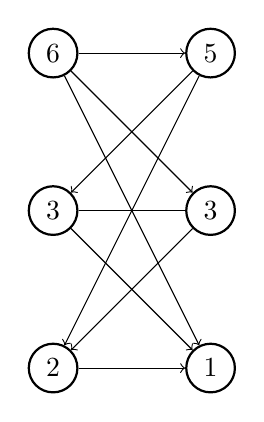
\begin{tikzpicture}
\begin{scope}[every node/.style={circle,thick,draw}]
  \node (1) at (0,0) {2};
  \node (2) at (0,2) {3};
  \node (3) at (0,4) {6};
  \node (4) at (2,0) {1};
  \node (5) at (2,2) {3};
  \node (6) at (2,4) {5};
\end{scope}

\draw[->] (1) -- (4); 
\draw[<-] (1) -- (5); 
\draw[<-] (1) -- (6); 
\draw[->] (2) -- (4); 
\draw[-] (2) -- (5); 
\draw[<-] (2) -- (6); 
\draw[->] (3) -- (4); 
\draw[->] (3) -- (5); 
\draw[->] (3) -- (6); 

\end{tikzpicture}
\label{fig:bipartite}
\caption{Dominance graph of $\{2,3,6\}$ vs. $\{1,3,5\}$}
\end{figure}

Another way to visualize hand $A$ against hand $B$ is a bipartite graph like Figure 3, counting ``right-pointing'' edges as +1, and ``left-pointing'' edges as -1. This shows that D($\{2,3,6\}$, $\{1,3,5\}) = 2$.



\section{Main Theorem and Proof Layout}

The main theorem we wish to prove states:

\begin{framed}
Given rational players, an optimal strategy in Dinosaur War is playing all options with uniform randomness.
\end{framed}

The steps to proving this are.

\begin{itemize}
\item Lemma 1: Across every row and column of the payoff matrix $M$ determined by hands $A$ and $B$, the entries sum to the graph's domination score $D(A,B)$.
\item Lemma 2: A payoff matrix of such a form of width $n$ has a Nash equilibrium\cite{2} of $p(a_i) = \frac{1}{n}, p(b_j) = \frac{1}{n}$ for all $i, j \in [1,n]$.
\item Lemma 3: The expected value of the game $A, B$ is then $\frac{D(A,B)}{n}$.
\end{itemize}

We will do this \emph{inductively} and \emph{simultaneously}, in that, if Lemma 1, 2, and 3 are true for boards of size $n-1$ and below, then we can prove them for a board of size $n$.

Additionally: There are no equilibria with a higher expected value in the game, since according to Von Neumann's Minimax theorem\cite{3}, all Nash equilibria of a zero-sum game have the same value. So though there may be other equally good strategies (duplicate cards in a hand allows the strategy to play \emph{one} versus the \emph{other} with some variation; also see the fait accompli games of Figure 2a, 2b), there are none more optimal than a uniform strategy.


Finally, we compute our payoff matrix for a larger game of card sets $A = B = [1,10]$.

\section{Lemmas: Base case}



\subsubsection{Base cases} 
\emph{Base case, n=1}: We see in Figure 4a that $D$ is equal to function $H$ at $n=1$: a 1 if player $A$'s single card outranks $B$'s, a 0 for a tie, and a $-1$ if $B$'s outranks. With a single element and therefore single row and column, the Lemma 1 is clearly true. There is only one total strategy in the game, so Lemma 2 is true. And Lemma 3 is equivalent to Lemma 1 when $n=1$.

\emph{(Extra) base case, n=2}: To see how this extends to a 2x2 matrix, consider Fig. 4b displaying the payoff matrix built from hands $A = (a_1, a_2) = \{3, 6\}; B = (b_1,b_2) = \{3,5\}$.

\begin{itemize}
\item The upper-left element is $T(a_1, b_1) + D(\{a_2\}, \{b_2\}) = T(a_1, b_1) + T(a_2, b_2)$
\item The upper-right element is $T(a_1, b_2) + D(\{a_2\}, \{b_1\}) = T(a_1, b_2) + T(a_2, b_1)$
\item The lower-left element is $T(a_2, b_1) + D(\{a_1\}, \{b_2\}) = T(a_2, b_1) + T(a_1, b_2)$
\item The lower-right element is $T(a_2, b_2) + D(\{a_1\}, \{b_1\}) = T(a_2, b_2) + T(a_1, b_1)$
\end{itemize}

It is clear that summing the top row, bottom row, left column, or right column yields $T(a_1, b_1) + T(a_1, b_2) + T(a_2, b_1) + T(a_2, b_2) = D(A,B)$. 

At the 2x2 size, it should be clear that:
\begin{itemize}
\item The upper left and lower right values are necessarily equal, as are the upper right and lower left. There are four possible game sequences (completely determined by the first move), and those starting with, say, $(3,3)$ in figure 5b need to end with $(6,5)$, equivalent to $[(6,5), (3,3)]$.
\item Because of this identity, the rows and columns all sum to the same value. (proving Lemma 1 at $n=2$)
\item An equilibrium strategy of this zero sum game is playing each option with probability $\frac{1}{2}$, as the players are essentially playing a game of Matching Pennies\cite{1} (showing Lemma 2).
\item Thefore, the expected payoff is the average of a(ny) row or column (showing Lemma 3).
\end{itemize}



\begin{figure}
\centering
\begin{subfigure}{.5\textwidth}
 \centering
 

$ \left[\begin{array}{cc}
            & \mathbf{5}\\ 
            \mathbf{6} & 1\\
           \end{array}\right] 
$

 \caption{1x1 base case}
\label{fig:basecase_1x1}
\end{subfigure}
\begin{subfigure}{.5\textwidth}
 \centering

$ \left[\begin{array}{ccc}
            & \mathbf{3} & \mathbf{5}\\ 
            \mathbf{3} & 1 & 0\\
            \mathbf{6} & 0 & 1\\
           \end{array}\right] 
$
 \caption{2x2 base case}
\label{fig:basecase_1x1}
\end{subfigure}
\caption{Base cases}
\label{fig:base}
\end{figure}


\section{Inductive case}



\begin{figure}
\centering
\begin{subfigure}{.5\textwidth}
 \centering
 
\[
\left[ 
\begin{array}{c@{}c@{}c@{}c}
& \mathbf{1} & \mathbf{3} & \mathbf{5} \\


\mathbf{2} & \left[\begin{array}{ccc}
            & \mathbf{3} & \mathbf{5}\\ 
            \mathbf{3} & 1 & 0\\
            \mathbf{6} & 0 & 1\\
           \end{array}\right] 
           & \left[\begin{array}{ccc}
            & \mathbf{1} & \mathbf{5}\\ 
            \mathbf{3} & 2 & 0 \\
            \mathbf{6} & 0 & 2 \\
           \end{array}\right]  
           & \left[\begin{array}{ccc}
            & \mathbf{1} & \mathbf{3}\\ 
            \mathbf{3} & 2 & 1 \\
            \mathbf{6} & 1 & 2 \\
           \end{array}\right]  \\           
           
 \mathbf{3} & \left[\begin{array}{ccc}
            & \mathbf{3} & \mathbf{5}\\ 
            \mathbf{2} &0 & 0 \\
            \mathbf{6} & 0 & 0 \\
           \end{array}\right]
           & \left[\begin{array}{ccc}
            & \mathbf{1} & \mathbf{5}\\ 
            \mathbf{2} & 2 & 0 \\
            \mathbf{6} & 0 & 2 \\
           \end{array}\right]  
           & \left[\begin{array}{ccc}
            & \mathbf{1} & \mathbf{3}\\ 
            \mathbf{2} & 2 & 0 \\
            \mathbf{6} & 0 & 2 \\
           \end{array}\right]  \\             
           
           
\mathbf{6} & \left[\begin{array}{ccc}
            & \mathbf{3} & \mathbf{5}\\ 
            \mathbf{2} & -2 & -1 \\
            \mathbf{3} & -1 & -2 \\
           \end{array}\right] 
& \left[\begin{array}{ccc}
            & \mathbf{1} & \mathbf{5}\\ 
            \mathbf{2} & 0 & 0 \\
            \mathbf{3} & 0 & 0 \\
           \end{array}\right]  
           & \left[\begin{array}{ccc}
            & \mathbf{1} & \mathbf{3}\\ 
            \mathbf{2} & 1 & 0 \\
            \mathbf{3} & 0 & 1 \\
           \end{array}\right]  \\  
\end{array}\right]
\]  
 \caption{Recursive game matrix}
\label{fig:236135_recursive}
\end{subfigure}

\begin{subfigure}{.5\textwidth}
\[
\left[ 
\begin{array}{c@{}c@{}c@{}c}
& \mathbf{1} & \mathbf{3} & \mathbf{5} \\


\mathbf{2} & (\mathit{1} + .5 = 1.5) & (\mathit{-1} + 1 = 0) & (\mathit{-1} + 1.5 = .5) \\
\mathbf{3} & (\mathit{1} +0 = 1) & (\mathit{0} + 1 = 1) & (\mathit{-1} + 1 = 0) \\             
 \mathbf{6} & (\mathit{1} + -1.5 = -.5) & (\mathit{1} + 0 = 1) & (\mathit{1} + .5 = 1.5) \\
\end{array}\right]
\]  
\caption{Payoff matrix}
\label{fig:236135_payoff}
\end{subfigure}

\caption{$\{2,3,6\}$ vs. $\{1,3,5\}$}
\label{fig:236135}
\end{figure}



For the \emph{inductive case}, consider Figure 5a and Figure 5b. In each, the vertical axis is the set of moves $A$ for player $P_A$, and the horizontal the move set $B$ for player $P_B$.

In Figure 5a, the element $(i,j)$ represents the game continuation (or subgame) should the next play be $(a_i, b_j)$ (so, excluding cards $a_i$ and $b_j$). 
In Figure 5b, the element $(i,j)$ is of the form (``immediate payoff from move $(a_i, b_j)$'' and ``expected payoff of remaining subgame''). So, the upper right element of 5b is $(\mathit{1} + .5 = 1.5)$; the italicized 1 represents that card 2 beats card 1. .5 points is the expected payoff of the subgame $\{3,6\}$ vs. $\{3,5\}$, totaling 1.5. 

\subsection{Inductive case for Lemma 1}

In 5a, the subgame at $(i, j)$ is the full game $(A - \{a_i\}, B-\{b_j\})$. This is ``the rest of the game'' with cards $a_i, b_j$ already used up. By inductive hypothesis, the payoff of the game at matrix entry $(1,1)$ is $D(A-\{a_i\}, B-\{b_j\})$, which is the sum of $T(a_m, b_n)$ for all combinations of $m, n$ except all those where $m=i$ or $n=j$. 

Without loss of generality, consider row $a_1$ ($P_A$ plays card 2) in Figure 5a (the subgames) and in figure 5b. Note that for $i=1$, summing across all expected subgame payoffs $\frac{D(A-\{a_1\}, B-\{b_j\})}{n-1}$ counts each pair $T(a_i, b_j), i \neq 1$ exactly $n-1$ times. $a_i, i \neq 1$ is always in each subgame, and $b_j$ is in every subgame except those in column $j$, for a total of $n-1$. So, with each $D$ term fully expanded, the sum includes $n-1$ terms $\frac{T(a_i, b_j)}{n-1}, i \neq 1$. These correspond to the numbers on the right side of the addition sign in figure 5b.

The immediate payoffs of playing $a_1$ (card 2 in this case) are just $T(a_1, b_1), T(a_1, b_2)... T(a_1, b_n)$, corresponding to the (italicized) number on the left side of the addition sign in 5b. Of course, summing the immediate payoffs ($\sum_{i=2}^n\sum_{j=1}^n T(a_i, b_j)$) and the subgame payoffs ($\sum_{j=1}^n T(a_1 b_j)$) is the definition of $D(A,B)$. This proves Lemma 1.

This logic holds equivalently for any other row or any column.

\subsection{Lemma 2}

Consider a payoff matrix where each row and each column sum to the same value (in our case, this is always $D(A,B)$).

A Nash equilibrium occurs for players $P_A, P_B$ when any deviation of $P_A$ from the equilibrium benefits $P_B$, assuming $P_A$ announces his strategy (and same for $P_B, P_A$).

Assume both strategies are uniform: $p(a_1) = p(a_2) = .... = \frac{1}{n} = p(b_1) = p(b_2) = ... p(b_n)$. Then the payoff of any given row $i$ would be, by Lemma 1, $\sum_{j=1}^n M_{i,j} = n \cdot \frac{1}{n} D(A,B) = D(A,B)$; the same follows for columns. The sum of all payoffs across the matrix is then $n \cdot D(A,B)$.

If $P_A$ shifts his strategy to a different distribution $p(a_1), p(a_2), ..., p(a_n)$, note that the sum of all payoffs $n\cdot D(A,B)$ does not change, since this is simply reallocating the probabilities, which sum to 1, over different rows each of expected value $D(A,B)$. 

\begin{itemize}
\item Case 1: If this reallocation sees each column $j$'s expected payoff $\sum_{i=1}^n M_{i,j} p(a_i)$  still summing to $D(A,B)$, then the equilibrium condition (and the same expected payoff) is maintained. 
\item Case 2: If, however, a column $j$ sums to a value greater than $D(A,B)$, then $p(b_j) = 1; p(b_k) = 0$ for $(k \neq j)$ increases $P_B$'s payoff. As a zero-sum game, this decreases $P_A$'s payoff, and $P_A$ would not choose it. Note that if Case 1 does not hold, there \emph{must} be a column like $j$, since the sum across all columns remains $n \cdot D(A,B)$. In other words, if we're not in Case 1, column sums can't all be less than or equal to $D(A,B)$, or the sum wouldn't be $n \cdot D(A,B)$, so at least one column has a payoff greater than $D(A,B)$.
\end{itemize}


With Lemma 2 proven, Lemma 3 follows quickly. Each $M_{i,j}$ occurs with probablity $\frac{1}{n^2}$, and the matrix entries sum to $n \cdot D(A,B)$, so the expected payoff is $\frac{D(A,B)}{n}$.




\section{Considerations and Examples}

Computing the expected value of the matrices in Figure 5a recursively gets computationally expensive, but with this formula in hand, the code \footnote{\url{https://github.com/fettermania/mathnotes/tree/main/dino/clj/dino/src/dino/core.clj}} becomes very simple: just apply Lemmas 1-3, and the 10 v. 10 game payoffs are easily generated (Figure 6).

Note that:

\begin{itemize}
\item The matrix is obviously symmetric.
\item Winning the first trick is neither a net positive nor negative.
\item Winning by exactly ($n/2$) rank spots is neutral; winning a trick by less than that yields a net positive value (for player $P_A$), and more than that, a negative value.
\end{itemize}
\begin{figure}
\centering
\setcounter{MaxMatrixCols}{20}

$\begin{bmatrix}
& \mathbf{1} & \mathbf{2} & \mathbf{3} & \mathbf{4} & \mathbf{5} & \mathbf{6} &\mathbf{7} & \mathbf{8} &\mathbf{9} & \mathbf{10} \\ 
\mathbf{1} & 0 & -8/9 & -2/3 & -4/9 & -2/9 & 0 & 2/9 & 4/9 & 2/3 & 8/9 \\
\mathbf{2} & 8/9 & 0 & -8/9 & -2/3 & -4/9 & -2/9 & 0 & 2/9 & 4/9 & 2/3 \\
\mathbf{3} & 2/3 & 8/9 & 0 & -8/9 & -2/3 & -4/9 & -2/9 & 0 & 2/9 & 4/9 \\
\mathbf{4} & 4/9 & 2/3 & 8/9 & 0 & -8/9 & -2/3 & -4/9 & -2/9 & 0 & 2/9 \\
\mathbf{5} & 2/9 & 4/9 & 2/3 & 8/9 & 0 & -8/9 & -2/3 & -4/9 & -2/9 & 0 \\
\mathbf{6} & 0 & 2/9 & 4/9 & 2/3 & 8/9 & 0 & -8/9 & -2/3 & -4/9 & -2/9 \\
\mathbf{7} & -2/9 & 0 & 2/9 & 4/9 & 2/3 & 8/9 & 0 & -8/9 & -2/3 & -4/9 \\
\mathbf{8} & -4/9 & -2/9 & 0 & 2/9 & 4/9 & 2/3 & 8/9 & 0 & -8/9 & -2/3 \\
\mathbf{9} & -2/3 & -4/9 & -2/9 & 0 & 2/9 & 4/9 & 2/3 & 8/9 & 0 & -8/9 \\
\mathbf{10} & -8/9 & -2/3 & -4/9 & -2/9 & 0 & 2/9 & 4/9 & 2/3 & 8/9 & 0 \\
\end{bmatrix}
$

\caption{$A = B = [1,10]$ payoff matrix}
\label{fig:236135}
\end{figure}


Though the double-uniform strategy is optimal, and no other perfect information strategies outperform it (Lemma 2), certainly, like \emph{Rock-Scissors-Paper}, having an inkling of what the opponent will do can yield advantage. 

Note again that there are cases where the choice of move truly does not matter, (like fig 2a and 2c), or, in some version of the game, where $k$ duplicate cards could render the choice between them irrelevant (as long as the sum of the probabilities remains $\frac{k}{n}$.

This paper has only dealt with the expected value of the game, not the chance of winning, though my intuition is that this would follow similarly\footnote{Though this is not a proof!}.



\begin{thebibliography}{9}
\bibitem{1} Wikipedia: \url{https://en.wikipedia.org/wiki/Matching_pennies}
\bibitem{2} Wikipedia: \url{https://en.wikipedia.org/wiki/Nash_equilibrium}
\bibitem{3} Wikipedia: \url{https://en.wikipedia.org/wiki/Minimax_theorem}
\end{thebibliography}

\end{comment}

\end{document}
